\chapter{Transient Analysis}
% TODO (possibly)
% Some material introducing the dielectrics inside a MOSFET transistor
% in order to motivate transients has been left out.
(For this lecture, a \textsc{mosfet} transistor is considered to transition between ``on'' and ``off'' at \(v_\text{GS} = \frac{1}{2} V_\text{DD}\).)

\begin{figure}
  \centering
  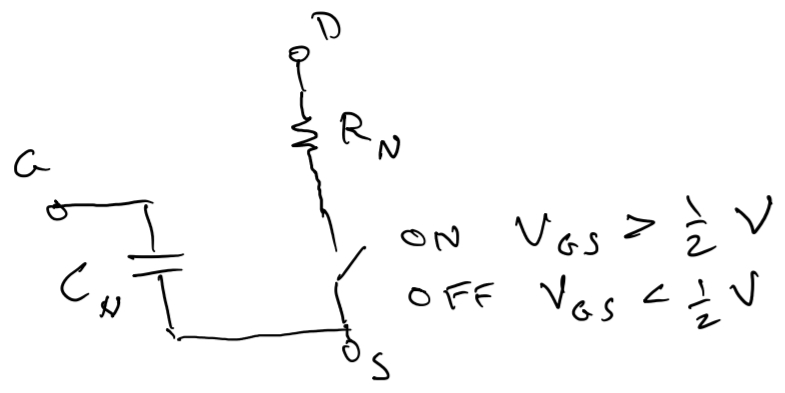
\includegraphics[width=0.75\linewidth]{figures/3/nmos-cap}
  \caption{Model of \textsc{nmos} transistor with G-S capacitance.}
  \label{figure:lec3-nmos-cap}
\end{figure}
\begin{figure}
  \centering
  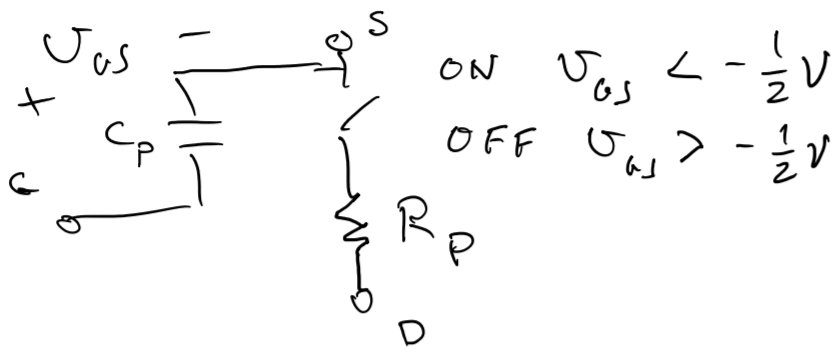
\includegraphics[width=0.75\linewidth]{figures/3/pmos-cap}
  \caption{Model of \textsc{pmos} transistor with G-S capacitance.}
  \label{figure:lec3-pmos-cap}
\end{figure}
We'll enrich our analog model of \textsc{mosfet}s as voltage-controlled switches by acknowledging capacitance between the \textsc{mosfet}'s gate and source.
\autoref{figure:lec3-nmos-cap} and \autoref{figure:lec3-pmos-cap}
depict \textsc{nmos} and \textsc{pmos} transistors in this model.

\begin{figure}
  \centering
  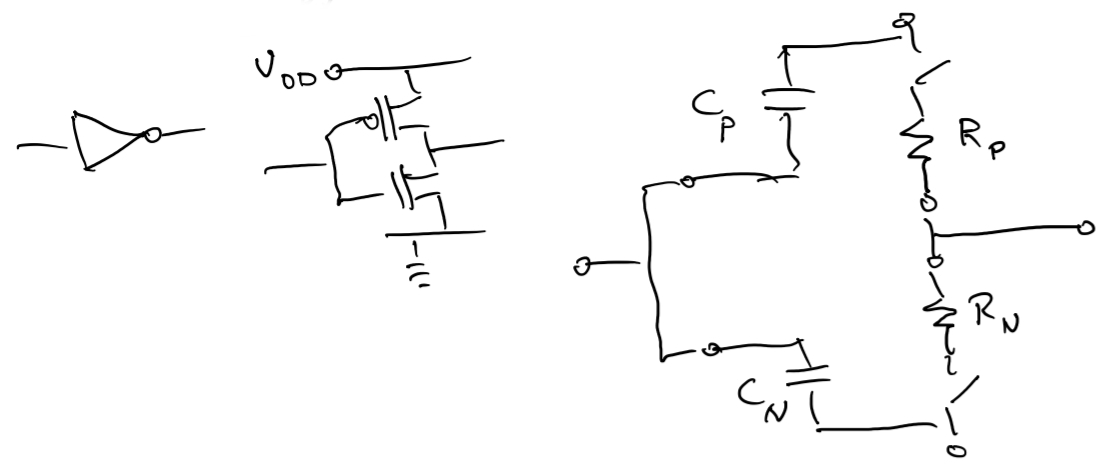
\includegraphics[width=0.75\linewidth]{figures/3/3inverters}
  \caption{A \textsc{cmos} inverter at three levels of abstraction.}
  \label{figure:lec3-3inverters}
\end{figure}
\autoref{figure:lec3-3inverters} summarizes the three levels of abstraction with which we are able to reason about \textsc{cmos} inverters.
On the very left is a digital symbol for an inverter that hides how the inverter works.
In the center is the construction of an inverter using complementary \textsc{mosfet}s.
On the right is a fairly faithful analog representation of an inverter that will allow us to interrogate the assumptions that, thus far, have enabled us to treat the analog circuit as a digital one.

\section{RC transient in an inverter chain}
Let's return to the case study of a chain of inverters, this time focusing on just two consecutive inverters.
\begin{figure}
  \centering
  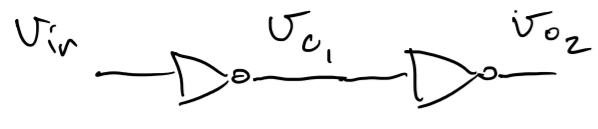
\includegraphics[width=0.75\linewidth]{figures/3/inverter-chain}
  \caption{Two consecutive \textsc{cmos} inverters, part of a longer chain.}
  \label{figure:lec3-inverter-chain}
\end{figure}
In \autoref{figure:lec3-inverter-chain} three wires are labeled as follows:
\begin{itemize}
  \item \(v_\text{in}\) is the input to the first inverter,
  \item \(v_{\text{o}_1}\) is the output of the first inverter (and the input to the second), and
  \item \(v_{\text{o}_2}\) is the output of the second.
\end{itemize}
The digital logic interpretation is that \(v_{\text{o}_2}\) is the double negation of \(v_\text{in}\), that is, \(v_{\text{o}_2} = v_\text{in}\).

\begin{figure}
  \centering
  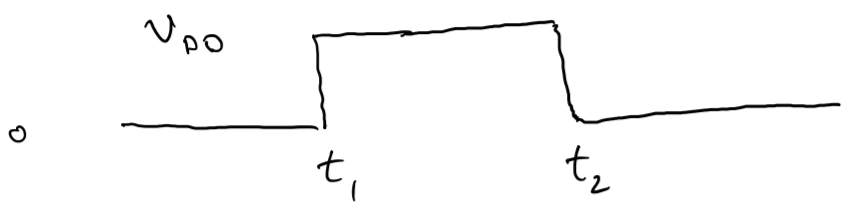
\includegraphics[width=0.75\linewidth]{figures/3/input-signal}
  \caption{Input signal to the first inverter of \autoref{figure:lec3-inverter-chain}}
  \label{figure:lec3-input-signal}
\end{figure}
We will study what happens when \(v_\text{in}\) is driven by the input depicted in \autoref{figure:lec3-input-signal}. It will begin having remained at 0 for a long time, change to \(v_\text{DD}\) at time \(t_1\), then return to \(0\) at time \(t_2 > t_1\).
\begin{figure}
  \centering
  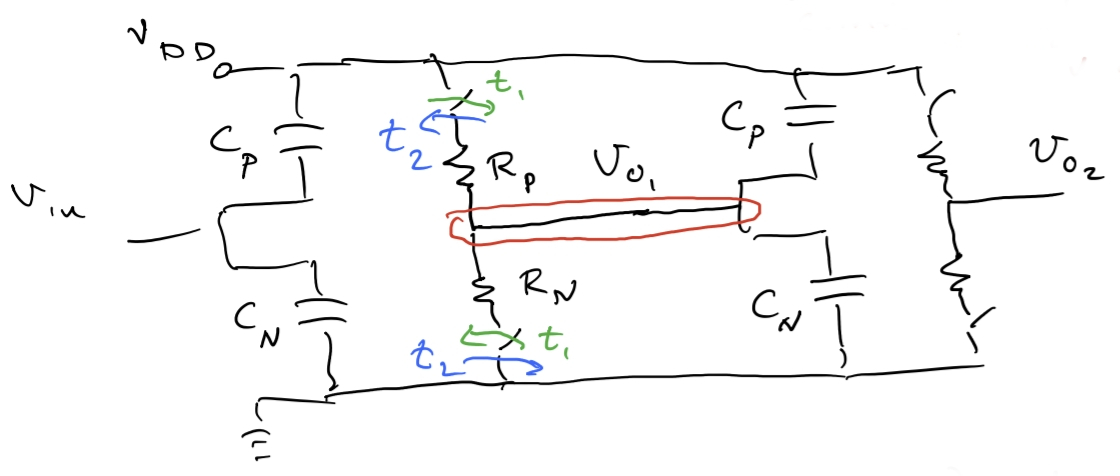
\includegraphics[width=1\linewidth]{figures/3/chain-RC}
  \caption{Analog redrawing of \autoref{figure:lec3-inverter-chain}, showing switch actions of the first inverter, as well as a distinguished node.}
  \label{figure:lec3-chain-RC}
\end{figure}
\autoref{figure:lec3-chain-RC} shows the actions of the switches of the first inverter's transistors at times \(t_1\) and \(t_2\).
For the rest of this section, we'll just concentrate on what happens to \(v_{\text{o}_1}\).

\subsection{Before \(t_1\)}
As \(v_\text{in} = 0\) well before \(t_1\), we can assume that the circuit has settled, and the output of the first inverter is \(v_\text{DD}\).

\subsection{After \(t_1\), before \(t_2\)}
At \(t_1\), the pull-up switch opens, and the pull-down switch closes.
KCL applied to the distinguished (red) middle node of \autoref{figure:lec3-chain-RC} requires the outgoing currents to sum to zero.
Using Ohm's Law once and the capacitor current-voltage relationship twice, we have the following equation:
\begin{align}
  \frac{v_{\text{o}_1}}{R_N}
  + C_N \dod{}{t} v_{\text{o}_1}
  + C_P \dod{}{t} \del{v_{\text{o}_1} - v_\text{DD}}
  &= 0 \\
  \dod{}{t} v_{\text{o}_1}
  + \frac{1}{R_N \del{C_N + C_P}} v_{\text{o}_1}
  &= 0\\
  \intertext{
  This is a differential equation that we will analyze with initial condition \(v_{\text{o}_1}(t_1) = V_\text{DD}\).
  For equations of this sort we will identify a characteristic quantity \(\tau\) as follows:
  }
  \tau &= R_N \del{C_N + C_P}
  \intertext{
  The International System of Units means that \(\tau\) is measured in Ohm-Farads, or seconds.
  For this reason, \(\tau\) is called the \emph{time constant} of the system.
  A time constant on the order of tens of picoseconds is considered state-of-the-art for modern devices, arising from resistances on the order of kiloOhms and capacitances on the order of femtofarads. Rewriting using \(\tau\),
  }
  \dod{}{t} v_{\text{o}_1}
  &= - \frac{1}{\tau} v_{\text{o}_1}\\
  \intertext{
  We will refer to the constant of proportionality between \(\od{}{t} v_{\text{o}_1}\) and \(v_{\text{o}_1}\) as \(\lambda\).
  }
  \dod{}{t} v_{\text{o}_1}
  &= \lambda v_{\text{o}_1}
  \intertext{
  There are many heuristic techniques to propose a solution to this differential equation. One of them is called Separation of Variables, which involves equations such as
  \(\int \frac{\dif v_{\text{o}_1}}{v_{\text{o}_1}} = \int \lambda \dif t\).
  The resulting solution form, where \(A\) is a constant that remains to be determined, is all that you will need to know about this variety of differential equation:
  }
  v_{\text{o}_1}(t)
  &= A e^{\lambda t}
  \intertext{
  (As an aside, you can verify that
  \(v_{\text{o}_1}(t) = A e^{\lambda t}\)
  is a solution---
  differentiating both sides with respect to \(t\) results in
  \(\od{}{t} v_{\text{o}_1}(t) = A \lambda e^{\lambda t} = \lambda (A e^{\lambda t})\).)
  Our next goal is to determine \(A\).
  We can do so by choosing \(A\) to meet the initial condition
  \(v_{\text{o}_1}(t_1) = V_\text{DD}\).
  Substituting \(v_{\text{o}_1}(t) = A e^{\lambda t}\),
  }
  A e^{\lambda t_1} &= V_\text{DD} \\
  A &= V_\text{DD} e^{-\lambda t_1} \\
  v_{\text{o}_1}
  &= \del{V_\text{DD} e^{-\lambda t_1}} e^{\lambda t} \\
  &= V_\text{DD} e^{-\del{\frac{t - t_1}{\tau}}}
\end{align}

\begin{figure}
  \centering
  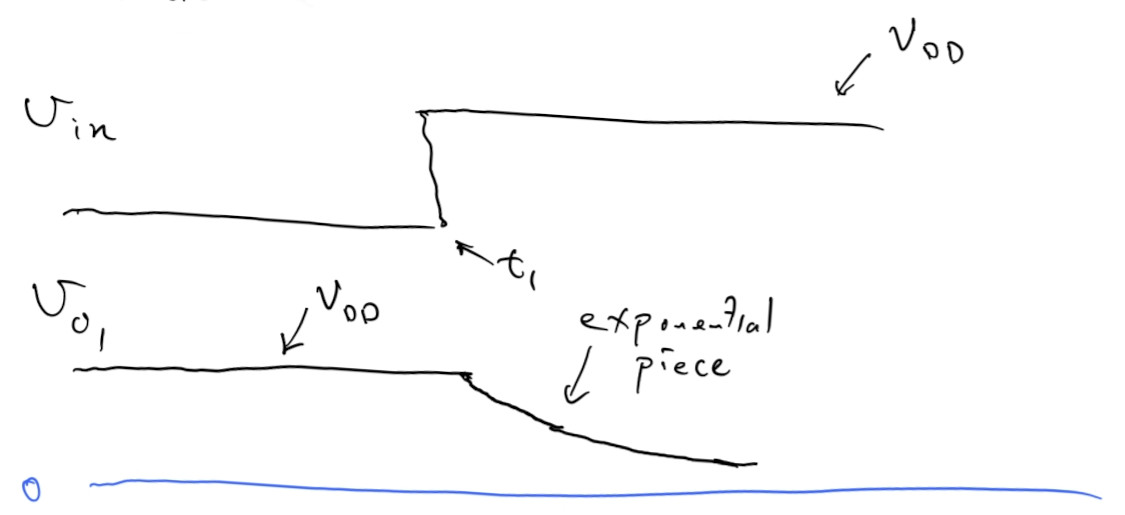
\includegraphics[width=\linewidth]{figures/3/exponential-sketch}
  \caption{Sketch of transient from \(t_1\) to \(t_2\) in \autoref{figure:lec3-chain-RC}.}
  \label{figure:lec3-transient}
\end{figure}
\autoref{figure:lec3-transient} is a sketch of \(v_\text{in}\) and \(v_{\text{o}_1}\) after \(t_1\) and before \(t_2\).
Notice that \(v_{\text{o}_1}\) doesn't immediately jump to \(0\) like the digital model assumes.
Rather, \(v_{\text{o}_1}\) decays exponentially toward 0 at a rate predicted by \(\tau\).
Discharging a capacitor takes time, and digital devices' clock speed is limited by how quickly binary values settle in between logic gates.


\subsection{After \(t_2\)}
We will try to write a differential equation describing the evolution of \(v_{\text{o}_1}\) at time \(t_2\) and beyond.
\autoref{figure:lec3-chain-RC} shows that at time \(t_2\), the pull-up switch closes, and the pull-down switch opens.
KCL applied to the same central node yields the following differential equation:
\begin{align}
  \frac{v_{\text{o}_1} - V_\text{DD}}{R_P}
  + \del{C_P + C_N} \dod{}{t} v_{\text{o}_1}
  &= 0\\
  \dod{}{t} v_{\text{o}_1}
  + \frac{1}{R_P\del{C_P + C_N}} v_{\text{o}_1}
  &= \frac{v_\text{DD}}{R_P \del{C_P + C_N}}
  \intertext{
  The previous solution for \(v_{\text{o}_1}\), which is valid up until time \(t_2\), may be evaluated at \(t_2\) for a boundary condition valid past \(t_2\):
  }
  v_{\text{o}_1}(t_2)
  &= V_\text{DD} e^{-\del{\frac{t_2 - t_1}{\tau}}}\\
  \intertext{
  A solution for \(v_{\text{o}_1}\) from \(t_2\) onwards is:
  }
  v_{\text{o}_1}
  &= V_\text{DD} + \del{v_{\text{o}_1}(t_2) - V_\text{DD}}
  e^{-\del{\frac{t - t_2}{\tau_P}}},
\end{align}
where \(\tau_P = R_P\del{C_P + C_N}\).
%% TODO: explain this?

\section{Uniqueness}
We solved a differential equation. Differential equations are universal and ubiquitous in science and engineering.

A theorem states that a large class of differential equations with boundary conditions have unique solutions. These differential equations are of the form
\begin{align}
  \dod{}{t} x
  &= f(x, t), \quad x(0) = x_0,
\end{align}
where
\begin{enumerate}
  \item
  for all values of \(t\), \(f(x, t)\) is differentiable with respect to \(x\) and
  \(\abs{ \pd{f}{x} (x,t) } < M\) for some nonnegative real number \(M\); and
  \item for all values of \(x\), \(f(x,t)\) has a finite number of discontinuities in \(t\) in any unit interval \([t_0, t_0 + 1]\).
\end{enumerate}
If these conditions hold, then our differential equation has a unique solution.

Note that these conditions are in fact quite loose, and are more than enough to certify that unique solutions exist to differential equations of the form \(\od{}{t} x = f(x) = \lambda x\).
It is important that we have proofs of existence and uniqueness because methods such as Separation of Variables are not inherently rigorous.
Only once we have verifed that a proposed solution satisfies the differential equation and boundary condition may we claim that it is a solution.
Because these problems have unique solutions, we may be certain that the model we are using is physically deterministic---it tells precisely what must happen, not just what \emph{may} happen.
